% !TEX encoding = UTF-8
% !TEX program = pdflatex
\documentclass[12pt]{article}

\usepackage[T2A]{fontenc}
\usepackage[utf8]{inputenc}
\usepackage[russian]{babel}
\usepackage{graphicx}
\textheight=24cm
\textwidth=16cm
\oddsidemargin=0pt
\topmargin=-1.5cm

\title{Лабораторная работа 3. 
Использование автоматических генераторов анализаторов Bison и ANTLR}
\author{\copyright~~Дарья Яковлева}
\date{01 мая 2016 года}
\begin{document}
\maketitle
\thispagestyle{empty}
Вариант 7. Хороший язык

Придумайте хороший императивный язык программирования, на
котором приятно писать программы. Транслируйте с него в Си.
Пример:

	\begin{verbatim}
		a, b = readint(), readint()
		a, b = b, a
		print(a + b)
	\end{verbatim}
Вывод:
	\begin{verbatim}
		int main() {
			int a, b;
			scanf("%d%d", a, b);
			int ta = a;
			int tb = b;
			a = tb;
			b = ta;
			printf("%d", a + b);
		}
	\end{verbatim}

\begin{itemize}
	\item \textbf{Транслятор}
		Translator.g4
	\begin{verbatim}
	\end{verbatim}
	\item \textbf{Примеры работы}
Пример 1.
Вход:
				\begin{verbatim}
					a = read_int()
					b = read_int()
					if (a > b) {
						a, b = b, a
					}
					c = 0
					for i = range(a, b) {
						c = c + i
					}
					print(c)
				\end{verbatim}
Вывод:
				\begin{verbatim}
					int a;					
					int b;					
					int c;					
					int i;					
					int main() {
						scanf("%d", &a);
						scanf("%d", &b);
						if (a>b) {
							int tmp = a;
							a = b;
							b = tmp;
						}
						c = 0;
						for (i = a; i < b; i++) {
							c = c+i;
						}
						printf("%d ", c);
					}
				\end{verbatim}
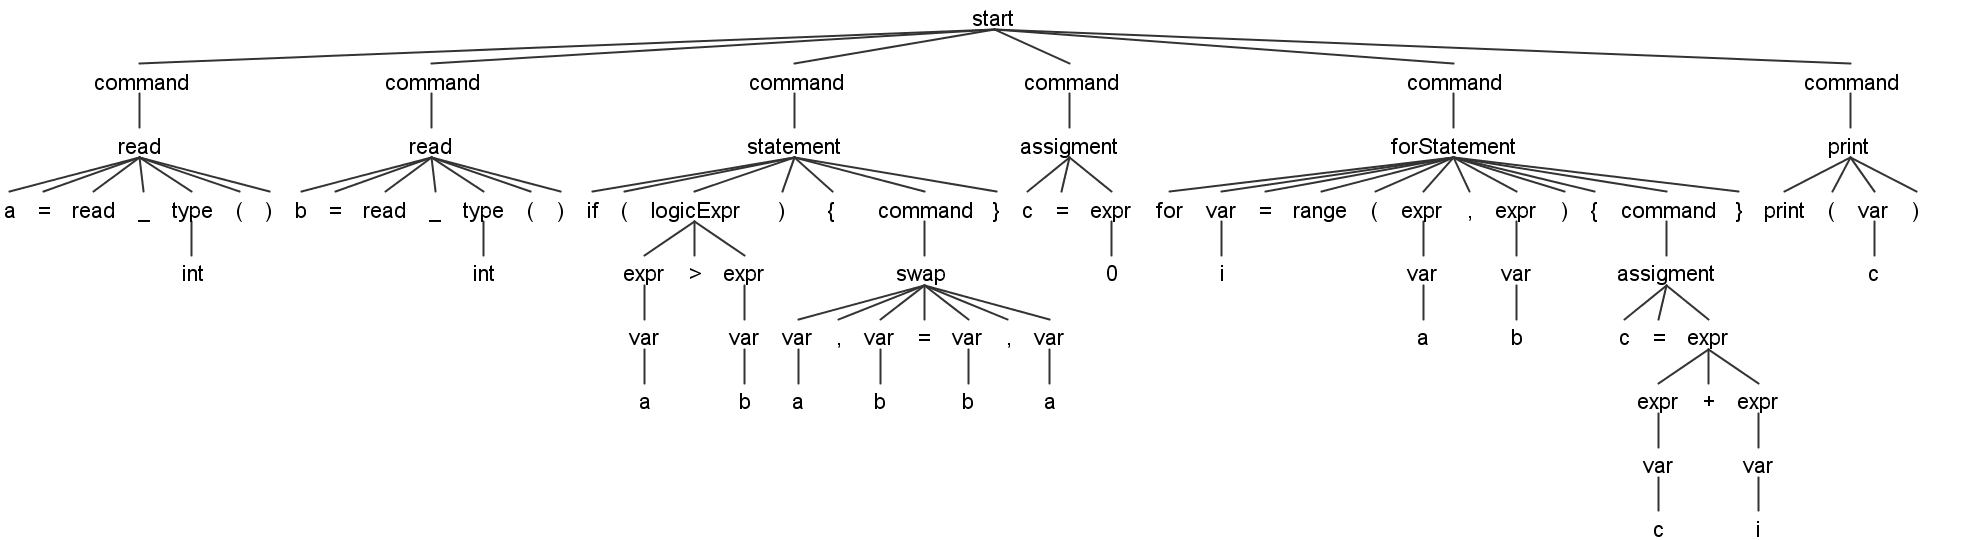
\includegraphics[width=15cm]{antlr4_parse_tree.png}			 

Пример 2.
Вход:
				\begin{verbatim}
					a = read_float()
					sqr = 0.0
					while (sqr * sqr < a) {
						sqr = sqr + 0.1
					}
					print('sqr is ')
					print(sqr)
				\end{verbatim}
Вывод:
				\begin{verbatim}
					float a;
					float sqr;
					int main() {
						scanf("%f", &a);
						sqr = 0.0;
						while (sqr*sqr<a) {
							sqr = sqr+0.1;
						}
						printf('sqr is ');
						printf("%f ", sqr);
					}
				
				\end{verbatim}
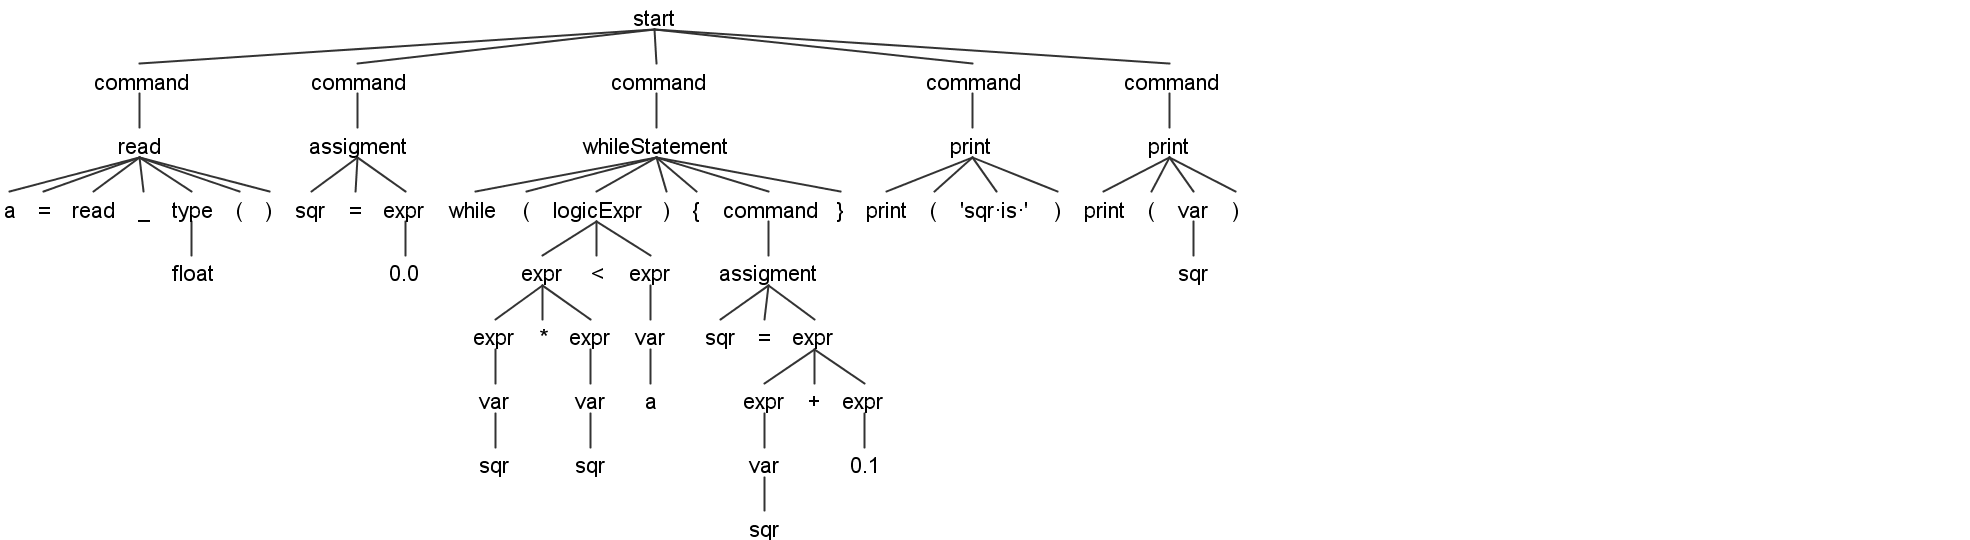
\includegraphics[width=25cm]{antlr4_parse_tree_1.png}			 
\end{itemize}

\end{document}

%%% Local Variables:
%%% fill-column: 10
%%% mode: latex
%%% coding: utf-8
%%% TeX-PDF-mode: t
%%% End: